% Copyright 2004 by Till Tantau <tantau@users.sourceforge.net>.
%
% In principle, this file can be redistributed and/or modified under
% the terms of the GNU Public License, version 2.
%
% However, this file is supposed to be a template to be modified
% for your own needs. For this reason, if you use this file as a
% template and not specifically distribute it as part of a another
% package/program, I grant the extra permission to freely copy and
% modify this file as you see fit and even to delete this copyright
% notice. 

\documentclass{beamer}

\usepackage[ngerman]{babel}
\usepackage[utf8]{inputenc}
\usepackage{graphics}
\usepackage{tikz}
\usepackage[decimalsymbol=comma]{siunitx}
\usepackage{amsmath}
\usepackage{ziffer}
\usepackage{scrextend}
\usepackage{color, colortbl}
\usepackage{ulem}
\usepackage{multicol}


% There are many different themes available for Beamer. A comprehensive
% list with examples is given here:
% http://deic.uab.es/~iblanes/beamer_gallery/index_by_theme.html
% You can uncomment the themes below if you would like to use a different
% one:
%\usetheme{AnnArbor}
%\usetheme{Antibes}
%\usetheme{Bergen}
%\usetheme{Berkeley}
%\usetheme{Berlin}
%\usetheme{Boadilla}
%\usetheme{boxes}
%\usetheme{CambridgeUS}
%\usetheme{Copenhagen}
%\usetheme{Darmstadt}
\usetheme{default}
%\usetheme{Frankfurt}
%\usetheme{Goettingen}
%\usetheme{Hannover}
%\usetheme{Ilmenau}
%\usetheme{JuanLesPins}
%\usetheme{Luebeck}
%\usetheme{Madrid}
%\usetheme{Malmoe}
%\usetheme{Marburg}
%\usetheme{Montpellier}
%\usetheme{PaloAlto}
%\usetheme{Pittsburgh}
%\usetheme{Rochester}
%\usetheme{Singapore}
%\usetheme{Szeged}
%\usetheme{Warsaw}

\newcommand*\conj[1]{\overline{#1}}
\newcommand*\oo{\infty}

\definecolor{tucinfo}{rgb}{0.49,0.6,0.16}
\definecolor{LightCyan}{rgb}{0.88,1,1}

\setbeamercolor{title}{fg=tucinfo}
\setbeamercolor{structure}{fg=tucinfo}


\title{cryptdomainmgr}

% A subtitle is optional and this may be deleted
\subtitle{automating Cert, TLSA, DKIM and many more}

\author{Stefan Helmert}
% - Give the names in the same order as the appear in the paper.
% - Use the \inst{?} command only if the authors have different
%   affiliation.

\institute[TU Chemnitz] % (optional, but mostly needed)
{
	Chaostreff Chemnitz
	
}


% - Use the \inst command only if there are several affiliations.
% - Keep it simple, no one is interested in your street address.

%\date{24.06.2017}
\date{\today}
% - Either use conference name or its abbreviation.
% - Not really informative to the audience, more for people (including
%   yourself) who are reading the slides online

\subject{Cryptdomainmgr}
% This is only inserted into the PDF information catalog. Can be left
% out. 

% If you have a file called "university-logo-filename.xxx", where xxx
% is a graphic format that can be processed by latex or pdflatex,
% resp., then you can add a logo as follows:

% \pgfdeclareimage[height=0.5cm]{university-logo}{university-logo-filename}
% \logo{\pgfuseimage{university-logo}}

% Delete this, if you do not want the table of contents to pop up at
% the beginning of each subsection:
%\AtBeginSubsection[]
%{
%  \begin{frame}<beamer>{Inhalt}
%    \tableofcontents[currentsection,currentsubsection]
%  \end{frame}
%}

% Let's get started
\begin{document}
	
	\begin{frame}
		\titlepage
	\end{frame}
	
	\begin{frame}{Content}
		\begin{multicols}{2}
		\tableofcontents
		\end{multicols}
		% You might wish to add the option [pausesections]
	\end{frame}
	
	% Section and subsections will appear in the presentation overview
	% and table of contents.
	\pagenumbering{arabic}
	
	\section{Motivation}
	\begin{frame}{\insertsection}{\insertsubsection}
		\textbf{$\rightarrow$ let's make a web app $\leftarrow$}
		\begin{itemize}
			\item DNS
			\item Webpage
			\item E-Mail
			\item Mailinglist
			\item \textbf{and the s for security}
		\end{itemize}
	\end{frame}
	
	\section*{DeMotivation}
	\begin{frame}{\insertsection}{\insertsubsection}
		\textbf{$\rightarrow$ let's make a web app $\leftarrow$}
		\begin{itemize}
			\item DNS
			\begin{itemize}
				\item SOA
				\item DNSSEC
			\end{itemize}
			\item Webpage
			\begin{itemize}
				\item HTTPS
				\item Certificate
				\item HSTS
				\item SRV
				\item TLSA
			\end{itemize}
			\item E-Mail
			\begin{itemize}
				\item Spam
				\item DKIM
				\item SPF
				\item ADSP
				\item DMARC
				\item SRV
			\end{itemize}
			\item Mailinglist
			\begin{itemize}
				\item SRS
			\end{itemize}
		\end{itemize}
	\end{frame}
	
	\subsection{fine}
	\begin{frame}{\insertsection}{\insertsubsection}
		\includegraphics[width=11cm]{CertOKen.png}
	\end{frame}

	\subsection{not so fine}
	\begin{frame}{\insertsection}{\insertsubsection}
		\includegraphics[height=8cm]{CertERRen.png}
	\end{frame}

	\section{Basics}
	\subsection{SSL Certifcate}
	\begin{frame}{\insertsection}{\insertsubsection}
		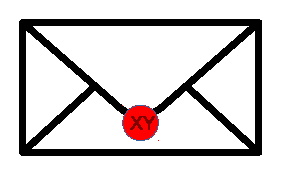
\includegraphics[height=3cm]{integrity.eps}
		\begin{itemize}
			\item authentication (phishing)
			\item integrity (man in the middle)
			\item privacy (spy)
		\end{itemize}
		$\rightarrow$ certbot renew
	\end{frame}
	
	\subsection{TLSA}
	\begin{frame}{\insertsection}{\insertsubsection}
		\textbf{DANE -- DNS-based Authentication of Named Entities}
		\textbf{Transport Layer Security Authentication} 
		\begin{itemize}
			\item locks certificate to domain/DNS (fraudulent CA, stolen cert)
		\end{itemize}
		$\rightarrow$ to do \\
		
		\textbf{CAA -- Certification Authority Authorization}
		\begin{itemize}
			\item specifies allowed CA
			\item checked by CA
		\end{itemize}
	\end{frame}	
	
	\subsection{DNSSEC}
	\begin{frame}{\insertsection}{\insertsubsection}
		\textbf{Domain Name System Security Extensions} 
		\begin{itemize}
			\item authenticate domain owner
			\item integrity (DNS cache poisoning)
		\end{itemize}
		$\rightarrow$ done by domain provider
	\end{frame}
	
	\subsection{DKIM}
	\begin{frame}{\insertsection}{\insertsubsection}
		\textbf{DomainKeys Identified Mail} 
		\begin{itemize}
			\item authenticate MTA (fake/spam server)
			\item integrity (man in the middle)
		\end{itemize}
		$\rightarrow$ to do
	\end{frame}

	\subsection{additional DNS records}
	\begin{frame}{\insertsection}{\insertsubsection}

		\textbf{SPF -- Sender Policy Framework} 
		\begin{itemize}
			\item which server is allowed to send email
		\end{itemize}
		\textbf{ADSP -- Author Domain Signing Practices}
		\begin{itemize}
			\item defines, if email must be DKIM signed
		\end{itemize}	
		\textbf{DMARC -- Domain-based Message Authentication, Reporting and Conformance}
		\begin{itemize}
			\item successor of SPF and ADSP
			\item overrides SPF and ADSP
			\item additional parameters: report email
		\end{itemize}
		\textbf{SRV -- Service}
		\begin{itemize}
			\item announces services
		\end{itemize}
	\end{frame}
		
	\section{Cryptdomainmgr}
	\subsection{autorenew process}
	\begin{frame}{\insertsection}{\insertsubsection}
		\begin{itemize}
			\item prepare
			\begin{itemize}
				\item generate certificate
				\item calculate TLSA from certificate
				\item add TLSA RR
				\item generate key pair for DKIM
				\item calculate DKIM
				\item add DKIM RR
			\end{itemize}
			\item rollover
			\begin{itemize}
				\item use new certificate
				\item use new DKIM key
			\end{itemize}
			\item cleanup
			\begin{itemize}
				\item remove old TLSA RR
				\item remove old DKIM RR
				\item delete old certificates
				\item delete old DKIM keys		
			\end{itemize}
		\end{itemize}
	\end{frame}
	

	\subsection{structure}
	\begin{frame}{\insertsection}{\insertsubsection}
		\begin{itemize}
			\item cryptdomainmgr
			\begin{itemize}
				\item dnsuptools
				\begin{itemize}
					\item domrobot
				\end{itemize}
				\item certbot
			\end{itemize}
		\end{itemize}
	\end{frame}	
	
\subsection{update cycle}
\begin{frame}[fragile]{\insertsection}{\insertsubsection} % fragiel: no indentation allowed
	\textbf{update -- set a, aaaa, srv, dmarc, spf, adsp}
	\begin{verbatim}
		~/cryptdomainmgr$ ./update.py inwxcred.conf example.conf
	\end{verbatim}
	\vspace{0.3cm}
	\textbf{prepare cycle -- generate Cert, TLSA, DKIM}
	\begin{verbatim}
	~/cryptdomainmgr$ ./prepare.py inwxcred.conf example.conf
	\end{verbatim}
	\vspace{0.3cm}
	\textbf{rollover cycle -- use Cert, TLSA, DKIM}
	\begin{verbatim}
	~/cryptdomainmgr$ ./rollover.py inwxcred.conf example.conf
	\end{verbatim}
	\vspace{0.3cm}
	\textbf{cleanup cycle -- remove outdated}
	\begin{verbatim}
	~/cryptdomainmgr$ ./cleanup.py inwxcred.conf example.conf
	\end{verbatim}
\end{frame}	

\section{Configuration}
\subsection{DNS credential}
\begin{frame}[fragile]{\insertsection}{\insertsubsection} % fragile: no indentation allowed
	\begin{verbatim}
	~/cryptdomainmgr$ cat inwxcred.conf
	
	[domain]
	user = myusername
	passwd = mypassword
	\end{verbatim}
\end{frame}		

\subsection{Certificates}
\begin{frame}[fragile]{\insertsection}{\insertsubsection} % fragile: no indentation allowed
	\begin{verbatim}
	~/cryptdomainmgr$ cat example.conf
	
	[certificate]
	generator = certbot
	email = stefan.helmert@t-online.de
	keysize = 4096
	
	[certificate:maincert]
	destination = /etc/ssl
	extraflags = --staging, --renew-with-new-domains, --hsts
	certname = fullchain.pem
	\end{verbatim}
	\begin{itemize}
		\item multiple domains using \texttt{maincert} $\rightarrow$ SAN certificate
	\end{itemize}
\end{frame}	

\subsection{DKIM}
\begin{frame}[fragile]{\insertsection}{\insertsubsection} % fragile: no indentation allowed
	\begin{verbatim}
	~/cryptdomainmgr$ cat example.conf
	
	[dkim]
	generator = rspamd
	
	[dkim:maindkim]
	signingConfTemplateFile = ~/cryptdomainmgr/dkim_signing_template.conf
	signingConfTemporaryFile = /etc/rspamd/dkim_signing_new.conf
	signingConfDestinationFile = /etc/rspamd/local.d/dkim_signing.conf
	\end{verbatim}
\end{frame}	
	
\subsection{Domain}
\begin{frame}[fragile]{\insertsection}{\insertsubsection} % fragile: no indentation allowed
	\begin{verbatim}
	~/cryptdomainmgr$ cat example.conf
	
	[domain]
	user = myusername
	handler = dnsuptools
	
	[domain:domain.example]
	soa.hostmaster = stefan.helmert@t-online.de
	soa.refresh = 7200
	
	[domain:sub.domain.example]
	ip4 = auto, 192.168.0.1
	ip6+ = auto, 0ffc::0030
	mx = mail20.domain.example:20, mail30.domain.example:30
	mx.40 = mail40.domain.example, mail50.domain.example:50
	mx.10+= mail10.domain.example
	\end{verbatim}
\end{frame}	

\begin{frame}[fragile]{\insertsection}{\insertsubsection} % fragile: no indentation allowed
	\textbf{set A record}
	\begin{verbatim}
	~/cryptdomainmgr$ cat example.conf
	
	[domain:sub.domain.example]
	ip4 = auto, 192.168.0.1
	\end{verbatim}
	means:
	\begin{itemize}
		\item add external ip and \texttt{192.168.0.1} to sub.domain.example
		\item delete all other A records of sub.domain.example
	\end{itemize}
\end{frame}	

\begin{frame}[fragile]{\insertsection}{\insertsubsection} % fragile: no indentation allowed
	\textbf{add A record}
	\begin{verbatim}
	~/cryptdomainmgr$ cat example.conf
	
	[domain:sub.domain.example]
	ip4+ = auto, 192.168.0.1
	\end{verbatim}
	means:
	\begin{itemize}
		\item add external ip and \texttt{192.168.0.1} to sub.domain.example
		\item \sout{delete all other A records of sub.domain.example}
	\end{itemize}
\end{frame}	

\begin{frame}[fragile]{\insertsection}{\insertsubsection} % fragile: no indentation allowed
	\textbf{set MX record}
	\begin{verbatim}
	~/cryptdomainmgr$ cat example.conf
	
	[domain:sub.domain.example]
	mx = mail20.domain.example:20, mail30.domain.example:30
	\end{verbatim}
	means:
	\begin{itemize}
		\item add MX records
		\begin{itemize}
			\item mail20.domain.example with prio 20
			\item mail30.domain.example with prio 30
		\end{itemize}
		\item delete all other MX records from sub.domain.example
	\end{itemize}
\end{frame}	

\begin{frame}[fragile]{\insertsection}{\insertsubsection} % fragile: no indentation allowed
	\textbf{set MX record}
	\begin{verbatim}
	~/cryptdomainmgr$ cat example.conf
		
	[domain:sub.domain.example]
	mx.40 = mail40.domain.example, mail50.domain.example:50
	\end{verbatim}
	means:
	\begin{itemize}
		\item add MX records
		\begin{itemize}
			\item mail40.domain.example with prio 40
			\item mail50.domain.example with prio 50
		\end{itemize}
		\item delete all other MX records with prio 40 from sub.domain.example
	\end{itemize}	
\end{frame}	

\begin{frame}[fragile]{\insertsection}{\insertsubsection} % fragile: no indentation allowed
	\textbf{set SRV record}
	\begin{verbatim}
	~/cryptdomainmgr$ cat example.conf
	
	[domain:sub.domain.example]
	srv.service.proto.port.weight.prio 
	= sub.domain.example:PRIO:WEIGHT:PORT:PROTO:SERVICE
	\end{verbatim}
\end{frame}	

\begin{frame}[fragile]{\insertsection}{\insertsubsection} % fragile: no indentation allowed
	\textbf{set DMARC entries}
	\begin{verbatim}
	~/cryptdomainmgr$ cat example.conf
	
	[domain:sub.domain.example]
	dmarc.p = quarantine
	dmarc.rua = mailto:stefan.helmert@t-online.de
	dmarc.ruf = mailto:stefan.helmert@gmx.net
	\end{verbatim}
	\begin{itemize}
		\item changes the entries \texttt{p}, \texttt{rua}, \texttt{ruf} of the \texttt{DMARC} record
		\item entries \texttt{adkim}, \texttt{aspf}, \texttt{pct} do not change
		\item "`atomic"' operation
		\item only one \texttt{DMARC} record allowed!
	\end{itemize}
\end{frame}	

\begin{frame}[fragile]{\insertsection}{\insertsubsection} % fragile: no indentation allowed
	\textbf{set DMARC record}
	\begin{verbatim}
	~/cryptdomainmgr$ cat example.conf
	
	[domain:sub.domain.example]
	dmarc =
	dmarc.p = quarantine
	dmarc.rua = mailto:stefan.helmert@t-online.de
	dmarc.ruf = mailto:stefan.helmert@gmx.net
	\end{verbatim}
	\begin{itemize}
		\item changes the entries \texttt{p}, \texttt{rua}, \texttt{ruf} of the \texttt{DMARC} record
		\item remove all other entries of this record
		\item "`atomic"' operation
		\item at most one \texttt{DMARC} record allowed!
	\end{itemize}
\end{frame}	

\begin{frame}[fragile]{\insertsection}{\insertsubsection} % fragile: no indentation allowed
	\textbf{set SOA entries}
	\begin{verbatim}
	~/cryptdomainmgr$ cat example.conf
	
	[domain:domain.example]
	soa.hostmaster = stefan.helmert@t-online.de
	soa.refresh = 7200
	\end{verbatim}
	\begin{itemize}
		\item changes the entries \texttt{hostmaster}, \texttt{refresh} of the \texttt{SOA} record
		\item \texttt{primns}, \texttt{serial}, \texttt{retry}, \texttt{expire}, \texttt{ncttl} not changed
		\item "`atomic"' operation
		\item exact one \texttt{SOA} record in top level allowed!
	\end{itemize}
\end{frame}	

\begin{frame}[fragile]{\insertsection}{\insertsubsection} % fragile: no indentation allowed
	\textbf{set SPF flags}
	\begin{verbatim}
	~/cryptdomainmgr$ cat example.conf
	
	[domain:domain.example]
	spf = -mx, a, ?all, +aaaa
	\end{verbatim}
	\begin{itemize}
		\item add given flags to \texttt{SPF} record
		\item remove all other flags from \texttt{SPF} record
		\item "`atomic"' operation
		\item at most one \texttt{SPF} record is allowed!
	\end{itemize}
\end{frame}	

\begin{frame}[fragile]{\insertsection}{\insertsubsection} % fragile: no indentation allowed
	\textbf{set ADSP and CAA records}
	\begin{verbatim}
	~/cryptdomainmgr$ cat example.conf
	
	[domain:domain.example]
	adsp = all
	caa =   0 issue letsdecrypt.org,
	      128 issuewild examplecert.example
	\end{verbatim}
	\begin{itemize}
		\item atomic update \texttt{ADSP} record
		\item add the \texttt{CAA} records
		\item remove all other \texttt{CAA} records
	\end{itemize}
\end{frame}	


\begin{frame}[fragile]{\insertsection}{\insertsubsection} % fragile: no indentation allowed
	\textbf{combine stuff -- TLSA and DKIM}
	\begin{verbatim}
	~/cryptdomainmgr$ cat example.conf

	[domain:sub.domain.example]	
	tlsa = 3 0 1, 3 1 1
	certificate = maincert
	dkim = maindkim
	\end{verbatim}
	\textbf{prepare cycle}
	\begin{itemize}
		\item add \texttt{TLSA} and \texttt{DKIM} records
	\end{itemize}
	\textbf{rollover cycle}
	\begin{itemize}
		\item no DNS changes
		\item apply certificates and keys on server
	\end{itemize}	\textbf{cleanup cycle}
	\begin{itemize}
		\item add \texttt{TLSA} and \texttt{DKIM} records (again)
		\item remove all other \texttt{TLSA} and \texttt{DKIM} records
	\end{itemize}	
\end{frame}	

\section{Implementation}
\subsection{cryptdomainmgr}
\begin{frame}[fragile]{\insertsection}{\insertsubsection} % fragile: no indentation allowed
	\begin{description}
		\item[cryptdomainmgr.py] core, brings everything together
		\item[cdmconfighandler.py] reads/interpretes config (ini) files
		\item[update.py] command line interface for generic DNS update
		\item[prepare.py] command line interface for prepare cycle
		\item[rollover.py] command line interface for rollover cycle
		\item[cleanup.py] command line interface for cleanup cycle
		\item[simplelogger/] logging abstraction, password $\rightarrow$ *****
		\item[dnsuptools/] domrobot interface abstraction, TLSA, DKIM calculation
	\end{description}	
\end{frame}	

\subsection{simplelogger} \label{sec:simplelogger}
\begin{frame}[fragile]{\insertsection}{\insertsubsection} % fragile: no indentation allowed
	\begin{description}
		\item[simplelogger.py] core, produces output
		\item[deepops.py] deep dict/list operations, password $\rightarrow$ *****
	\end{description}	
\end{frame}	

\subsection{dnsuptools}
\begin{frame}[fragile]{\insertsection}{\insertsubsection} % fragile: no indentation allowed
	\begin{description}
		\item[dnsuptools.py] core, high level, record change \& query methods
		\item[dnsupdate.py] interface to domrobot, low level
		\item[dkimrecgen.py] reads/interpretes dkim key file
		\item[tlsarecgen.py] reads/interpretes certificate file
		\item[simplelogger/] see simplelogger \ref{sec:simplelogger}
		\item[inwxclient/] domrobot client
	\end{description}	
\end{frame}	

\section{Discussion}
\begin{frame}[fragile]{\insertsection}{\insertsubsection} % fragile: no indentation allowed
  \Huge{???}	
\end{frame}	

\end{document}





